\documentclass[11pt,a4paper]{article}
\usepackage[a4paper,top=25mm,bottom=23mm,left=22mm,right=22mm]{geometry}
\usepackage{graphicx,xcolor,booktabs,tabularx,fancyhdr}
\usepackage{tikz}
\usetikzlibrary{arrows.meta,positioning}
\usepackage[colorlinks=true,linkcolor=black,urlcolor=teal,pdftitle={Artaud - Mini Distributed Object Store},pdfsubject={Cloud computing project report}]{hyperref}

\definecolor{ink}{HTML}{162C25}
\definecolor{forest}{HTML}{17634D}
\definecolor{slate}{HTML}{40544B}
\definecolor{mist}{HTML}{EAF3EF}
\definecolor{linegreen}{HTML}{B9D2C7}
\definecolor{paperwhite}{HTML}{F6F9F7}

\setlength{\parindent}{0pt}
\setlength{\parskip}{7pt}
\setlength{\headheight}{16pt}
\setlength{\emergencystretch}{2em}
\renewcommand{\arraystretch}{1.22}
\frenchspacing
\pagestyle{fancy}
\fancyhf{}
\fancyhead[L]{\small\textsf{\textcolor{forest}{ARTAUD}}}
\fancyhead[R]{\small\textsf{\textcolor{slate}{CLOUD COMPUTING PROJECT}}}
\fancyfoot[L]{\small\textsf{\textcolor{slate}{MINI DISTRIBUTED OBJECT STORE}}}
\fancyfoot[R]{\small\textsf{\textcolor{forest}{\thepage}}}
\renewcommand{\headrulewidth}{0.35pt}

\newcommand{\reportsection}[1]{%
  \par\noindent{\huge\sffamily\bfseries\color{ink}#1}\par
  \vspace{1mm}{\color{linegreen}\rule{\linewidth}{0.6pt}}\par}
\newcommand{\topic}[1]{\par\medskip{\large\sffamily\bfseries\color{forest}#1}\par}
\newcommand{\code}[1]{\texttt{#1}}
\newcommand{\figcaption}[2]{%
  \par{\small\sffamily\color{slate}\textbf{Figure #1.} #2}\par}
\newcommand{\testedcommit}{20357e2}
\newcommand{\repo}{https://github.com/KiritoReborn/mini-object-store}
\newcommand{\keyfact}[2]{%
  \begin{minipage}[t]{0.29\linewidth}
    {\huge\sffamily\bfseries\color{forest}#1}\par
    {\small\sffamily\color{slate}#2}
  \end{minipage}}

\begin{document}

\thispagestyle{empty}
\noindent{\color{forest}\rule{\linewidth}{1.4pt}}\par
\vspace{10mm}
{\large\sffamily\bfseries\color{forest} CLOUD COMPUTING PROJECT REPORT}\par
\vspace{15mm}
\scalebox{2.05}{{\Huge\sffamily\bfseries\color{ink}Artaud}}\par
{\LARGE\sffamily\color{slate} Mini Distributed Object Store}\par
\vspace{14mm}
{\large
A storage service that splits uploaded files across four Docker workers,
checks every chunk before serving a download, and restores redundancy after
a worker outage or detected replica damage. A browser dashboard exposes
placement and recovery during the local demo.\par}
\vspace{11mm}

\noindent\colorbox{mist}{\parbox{\dimexpr\linewidth-2\fboxsep\relax}{%
  \vspace{6mm}\hspace{4mm}
  \keyfact{4}{storage workers}\hfill
  \keyfact{2}{copies per chunk}\hfill
  \keyfact{1 MB}{default chunk size}
  \vspace{6mm}}}

\vspace{11mm}
\topic{Project scope}
The local stack implements the six object endpoints in the assignment and
ships a console for uploads, worker visibility, replica inspection and
controlled fault demonstrations. The controller owns object metadata and
orchestration. Workers own the persistent chunk bytes.

\vfill
\noindent{\color{linegreen}\rule{\linewidth}{0.6pt}}\par
{\small\sffamily\color{slate} 23 November 2026 \hfill
  \href{\repo/tree/20357e2c03212e9e3d8765286f69cbbbbfe62233}{Source snapshot \testedcommit}}

\clearpage
\reportsection{System architecture}

Clients use a single HTTP endpoint on port 8000. The controller coordinates
object operations and writes metadata to SQLite. Workers communicate over the
private Compose network and persist chunks and checksum sidecars in separate
named volumes. The controller volume also contains temporary files used during
download verification.

\begin{center}
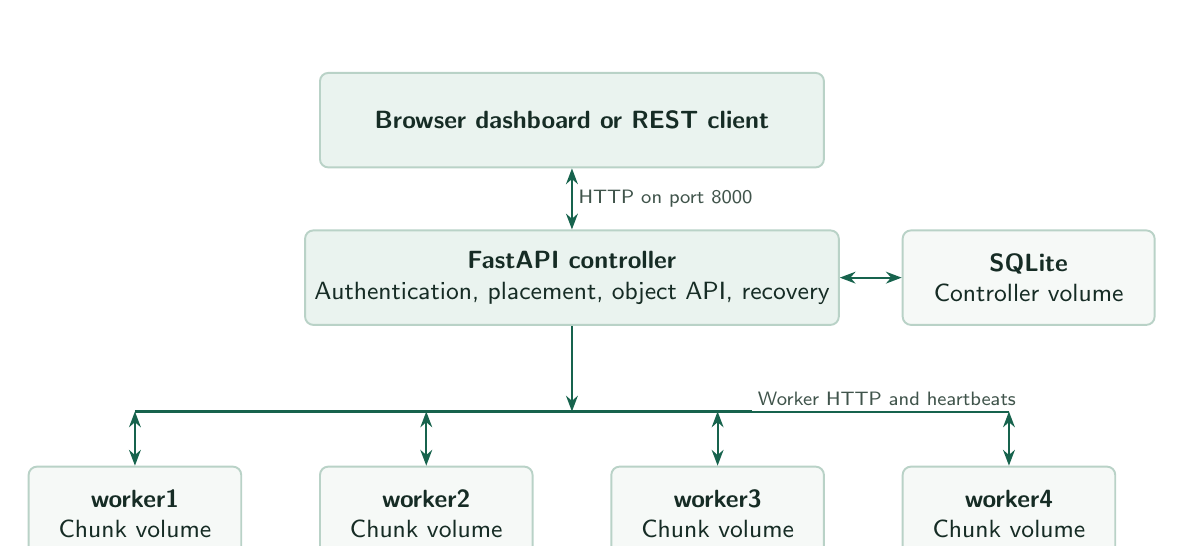
\begin{tikzpicture}[
  font=\small\sffamily,
  box/.style={draw=linegreen, line width=.7pt, rounded corners=3pt,
    fill=paperwhite, text=ink, align=center, minimum height=12mm,
    minimum width=27mm},
  central/.style={box, fill=mist, minimum width=64mm},
  route/.style={-{Stealth[length=2mm]}, line width=.8pt, draw=forest},
  both/.style={{Stealth[length=2mm]}-{Stealth[length=2mm]},
    line width=.8pt, draw=forest},
  labeltext/.style={text=slate, font=\scriptsize\sffamily, fill=white,
    inner sep=2pt}
]
\node[central] (client) at (0,0) {\textbf{Browser dashboard or REST client}};
\node[central] (controller) at (0,-2.0)
  {\textbf{FastAPI controller}\\Authentication, placement, object API, recovery};
\node[box, minimum width=32mm] (db) at (5.8,-2.0)
  {\textbf{SQLite}\\Controller volume};
\node[box] (w1) at (-5.55,-5.0) {\textbf{worker1}\\Chunk volume};
\node[box] (w2) at (-1.85,-5.0) {\textbf{worker2}\\Chunk volume};
\node[box] (w3) at (1.85,-5.0) {\textbf{worker3}\\Chunk volume};
\node[box] (w4) at (5.55,-5.0) {\textbf{worker4}\\Chunk volume};
\draw[both] (client) -- node[labeltext,right]{HTTP on port 8000} (controller);
\draw[both] (controller) -- (db);
\draw[route] (controller.south) -- (0,-3.7);
\draw[draw=forest,line width=.8pt] (-5.55,-3.7) -- (5.55,-3.7);
\foreach \x/\w in {-5.55/w1,-1.85/w2,1.85/w3,5.55/w4}{
  \draw[both] (\x,-3.7) -- (\w.north);
}
\node[labeltext,anchor=south] at (4.0,-3.7) {Worker HTTP and heartbeats};
\end{tikzpicture}
\end{center}
\figcaption{1}{The controller routes client requests, replica transfers and repairs.}

\topic{Implementation and ownership}
\begin{tabularx}{\linewidth}{@{}p{29mm}X@{}}
\toprule
\textbf{Responsibility} & \textbf{Implementation} \\
\midrule
Member A & Controller object API, metadata and placement, browser dashboard and operator controls. \\
Member B & Worker HTTP service, disk storage, heartbeat, verified admission and recovery. \\
Shared & Controller--worker contracts, Compose topology, integration verification and the demo. \\
\bottomrule
\end{tabularx}

\topic{Access}
The base stack binds to the local host. When the owner key is configured,
clients send it in \code{X-Artaud-Key}. The demo overlay adds worker container
controls and fault injection. The assignment demonstration uses the local
stack, while the repository documents Vercel separately for remote presentations.

\clearpage
\reportsection{Object lifecycle and API}

\topic{Upload and placement}
The controller reads the incoming file in chunks of up to 1,000,000 bytes and
computes SHA-256 digests. Placement picks two distinct eligible workers using
recorded chunk count, then worker ID to break ties. Choosing by chunk count
can even out replica counts while total bytes differ because tail chunks are
often smaller. The controller publishes the object as \code{READY} after all
required writes succeed. A failed upload can retry a worker write or fail
without exposing a partial object as ready.

\topic{Reads, metadata and deletion}
The controller resolves the manifest, checks each candidate copy against the
expected size and digest in SQLite and retries another copy when needed.
It assembles and verifies the object in a temporary file before sending
binary bytes. If a chunk has no verified readable copy, the download returns
a JSON \code{503}. A valid range can select bytes from the verified file.

Custom metadata is updated separately from immutable system fields. Deleting
an object removes it from public listings and works through physical replica
cleanup. Reconciliation can resume interrupted deletion.

\topic{Required HTTP operations}
\begin{tabularx}{\linewidth}{@{}l l X r@{}}
\toprule
\textbf{Method} & \textbf{Path suffix} & \textbf{Purpose} & \textbf{Success} \\
\midrule
\code{POST} & (collection) & Upload a file and optional JSON metadata & 201 \\
\code{GET} & (collection) & List ready objects & 200 \\
\code{GET} & \code{/\{id\}} & Download the original bytes & 200 \\
\code{GET} & \code{/\{id\}/metadata} & Read system and custom metadata & 200 \\
\code{PATCH} & \code{/\{id\}/metadata} & Merge custom metadata fields & 200 \\
\code{DELETE} & \code{/\{id\}} & Remove the object & 204 \\
\bottomrule
\end{tabularx}

\smallskip
The collection URL is \code{/api/v1/objects}. Uploads use
\code{multipart/form-data} with a \code{file} field and optional
\code{metadata} field. Invalid requests use JSON errors, including
\code{400} for invalid input and \code{404} for unknown objects.

\topic{Integrity boundary}
SQLite is the authority for expected hashes. Worker sidecars support local
disk verification. The acceptance test changes both the chunk bytes and the
local sidecar, then verifies that the controller still identifies the
mismatch and restores the expected content.

\clearpage
\reportsection{Failure detection and repair}

Workers register in \code{JOINING}. Registration and inventory verification
precede admission as \code{ALIVE}. By default, workers send heartbeats every
five seconds, and a heartbeat becomes stale after 15 seconds. The recovery
loop runs every five seconds and periodically verifies inventory and bytes on
live workers.

\begin{center}
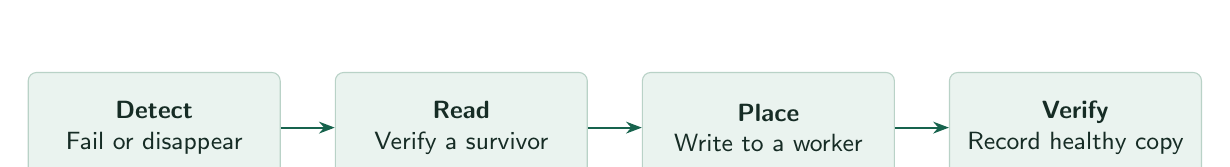
\begin{tikzpicture}[
  stage/.style={draw=linegreen, fill=mist, rounded corners=3pt, align=center,
    text=ink, font=\small\sffamily, minimum width=32mm, minimum height=14mm},
  flow/.style={-{Stealth[length=2mm]}, draw=forest, line width=.8pt}]
\node[stage] (detect) at (0,0) {\textbf{Detect}\\Fail or disappear};
\node[stage] (read) at (3.9,0) {\textbf{Read}\\Verify a survivor};
\node[stage] (write) at (7.8,0) {\textbf{Place}\\Write to a worker};
\node[stage] (check) at (11.7,0) {\textbf{Verify}\\Record healthy copy};
\draw[flow] (detect) -- (read);
\draw[flow] (read) -- (write);
\draw[flow] (write) -- (check);
\end{tikzpicture}
\end{center}
\figcaption{2}{Replica repair requires a verified source and a separate eligible destination. Returning workers can reintroduce valid copies, which can be trimmed after two other copies have been verified.}

\topic{What the dashboard means}
\begin{tabularx}{\linewidth}{@{}p{29mm}X@{}}
\toprule
\textbf{State} & \textbf{Interpretation} \\
\midrule
\code{HEALTHY} & The recorded replica passed a verification check. \\
\code{MISSING} & The worker does not have the expected chunk. \\
\code{CORRUPT} & The observed bytes failed the expected size or digest check. \\
\code{DEAD} & A worker state derived from stale heartbeats. Its persisted bytes may remain on disk. \\
\bottomrule
\end{tabularx}

\topic{Failure outcomes}
When one of two holders goes offline, reads can fall back to the second holder
while repair restores two-copy redundancy on eligible workers. If both holders
of the same chunk are unavailable before repair takes place, downloads of
that object return \code{503} until a verified copy returns. Restarting a
worker preserves its named volume. Losing both valid copies permanently
requires restoring the original bytes from a backup.

\topic{Deployment limits}
All five containers share one host. A host or disk failure can affect the
whole stack. The single controller and SQLite database are also shared
dependencies. The 50 MB check establishes end-to-end correctness at that
size. The project did not measure storage throughput or peak memory.

\clearpage
\reportsection{Difficulties faced during development}

\topic{Distinguishing failure scenarios}
Recovery was the most challenging part of the project because similar
symptoms could have different causes. A chunk could be absent from disk,
present with damaged bytes, or temporarily unreachable because its worker
was offline. We encountered these distinctions when we began combining
failures during deployment and testing. An absent chunk is marked
\code{MISSING} and a failed integrity check can mark a copy
\code{CORRUPT}. A worker outage is tracked separately so a timeout does
not cause valid data to be discarded.

\topic{Separating fault injection from detection}
Our first version of \textbf{Corrupt this copy} immediately marked the
replica as \code{CORRUPT}. The dashboard showed corruption followed by
repair, so we initially took that as evidence of detection. The demo
action itself had supplied the diagnosis. A successful injection now
changes one stored byte and records the action. A later download or
background scan verifies the copy and can independently classify it as
damaged.

\topic{Detecting damage after a successful download}
A successful download could hide a damaged replica. When the controller
read the healthy copy first, the user got the correct file even though
only one valid copy remained. We added periodic verification of live
workers' stored copies against the controller's checksums. Heartbeats tell
us whether a worker has communicated recently. Inventory and checksum
checks tell us which expected chunks it has and whether their bytes
match.

\topic{Reconciling a worker that returns}
After roughly 15 seconds without a heartbeat, the controller can mark a
worker \code{DEAD} and use surviving valid copies to restore redundancy.
When the worker returns, the controller checks its actual inventory before
readmission. An expected chunk may be missing, a returning copy may be
the only surviving source, or repair may already have created two healthy
copies elsewhere. The controller can remove a surplus copy once it
verifies two others. If both copies of a required chunk are damaged and
no verified source survives, the affected object remains unavailable until
valid data is restored.

The recovery tests check the evidence behind each outcome, including
how damage was detected, the number of valid copies after repair, and
what changed when the offline worker returned.

\clearpage
\reportsection{Consistency and file transfers}

\topic{Publishing complete uploads}
A worker can fail after receiving some chunks or between writes of the
same chunk. The controller keeps the object in \code{UPLOADING} while
it places replicas and exposes it only after the database can commit
\code{READY}. A failed or cancelled upload goes through cleanup, and
uncertain writes can remain tracked for a later attempt. API tests force
a failed upload and check that clients cannot list or download the
incomplete object.

\topic{Verifying a download before sending it}
A missing chunk discovered halfway through a download would otherwise
leave the client with a partial file and an HTTP success status. The
controller builds the file in temporary disk storage one verified chunk
at a time and checks the whole-object hash before sending a response.
This design uses temporary disk space and adds preparation time before
the client receives bytes. Tests check that an unreadable object returns
a JSON \code{503} and cleans up its temporary file. The live run also
compares the original and retrieved hashes for a 50 MB file.

\topic{Coordinating uploads, repairs and deletions}
Cleanup during an upload could mistake its chunks for abandoned data.
At the same time, repair could place a replacement while another request
was deleting the file. The controller uses a lock per object and rereads
the relevant state after taking the lock. It protects active uploads and
can retry cleanup when a worker that missed deletion returns. Tests
exercise an inventory scan waiting for an upload, deletion waiting for
repair, and recovery of an interrupted delete.

\topic{Diagnosing the hosted dashboard connection}
Vercel could serve the dashboard even when the controller on our PC
was unreachable. We kept the controller's HTTPS address configurable
in the browser, with a connection test and a separate owner key field.
The remote dashboard sends API requests directly to the controller
through the tunnel, and the controller allows requests from configured
browser origins. The local dashboard uses the same origin as the API,
so the local demonstration can run without the tunnel.

\clearpage
\reportsection{Dashboard walkthrough}

\begingroup
\setlength{\fboxsep}{0pt}
\setlength{\fboxrule}{0.5pt}
\begin{center}
\fcolorbox{linegreen}{white}{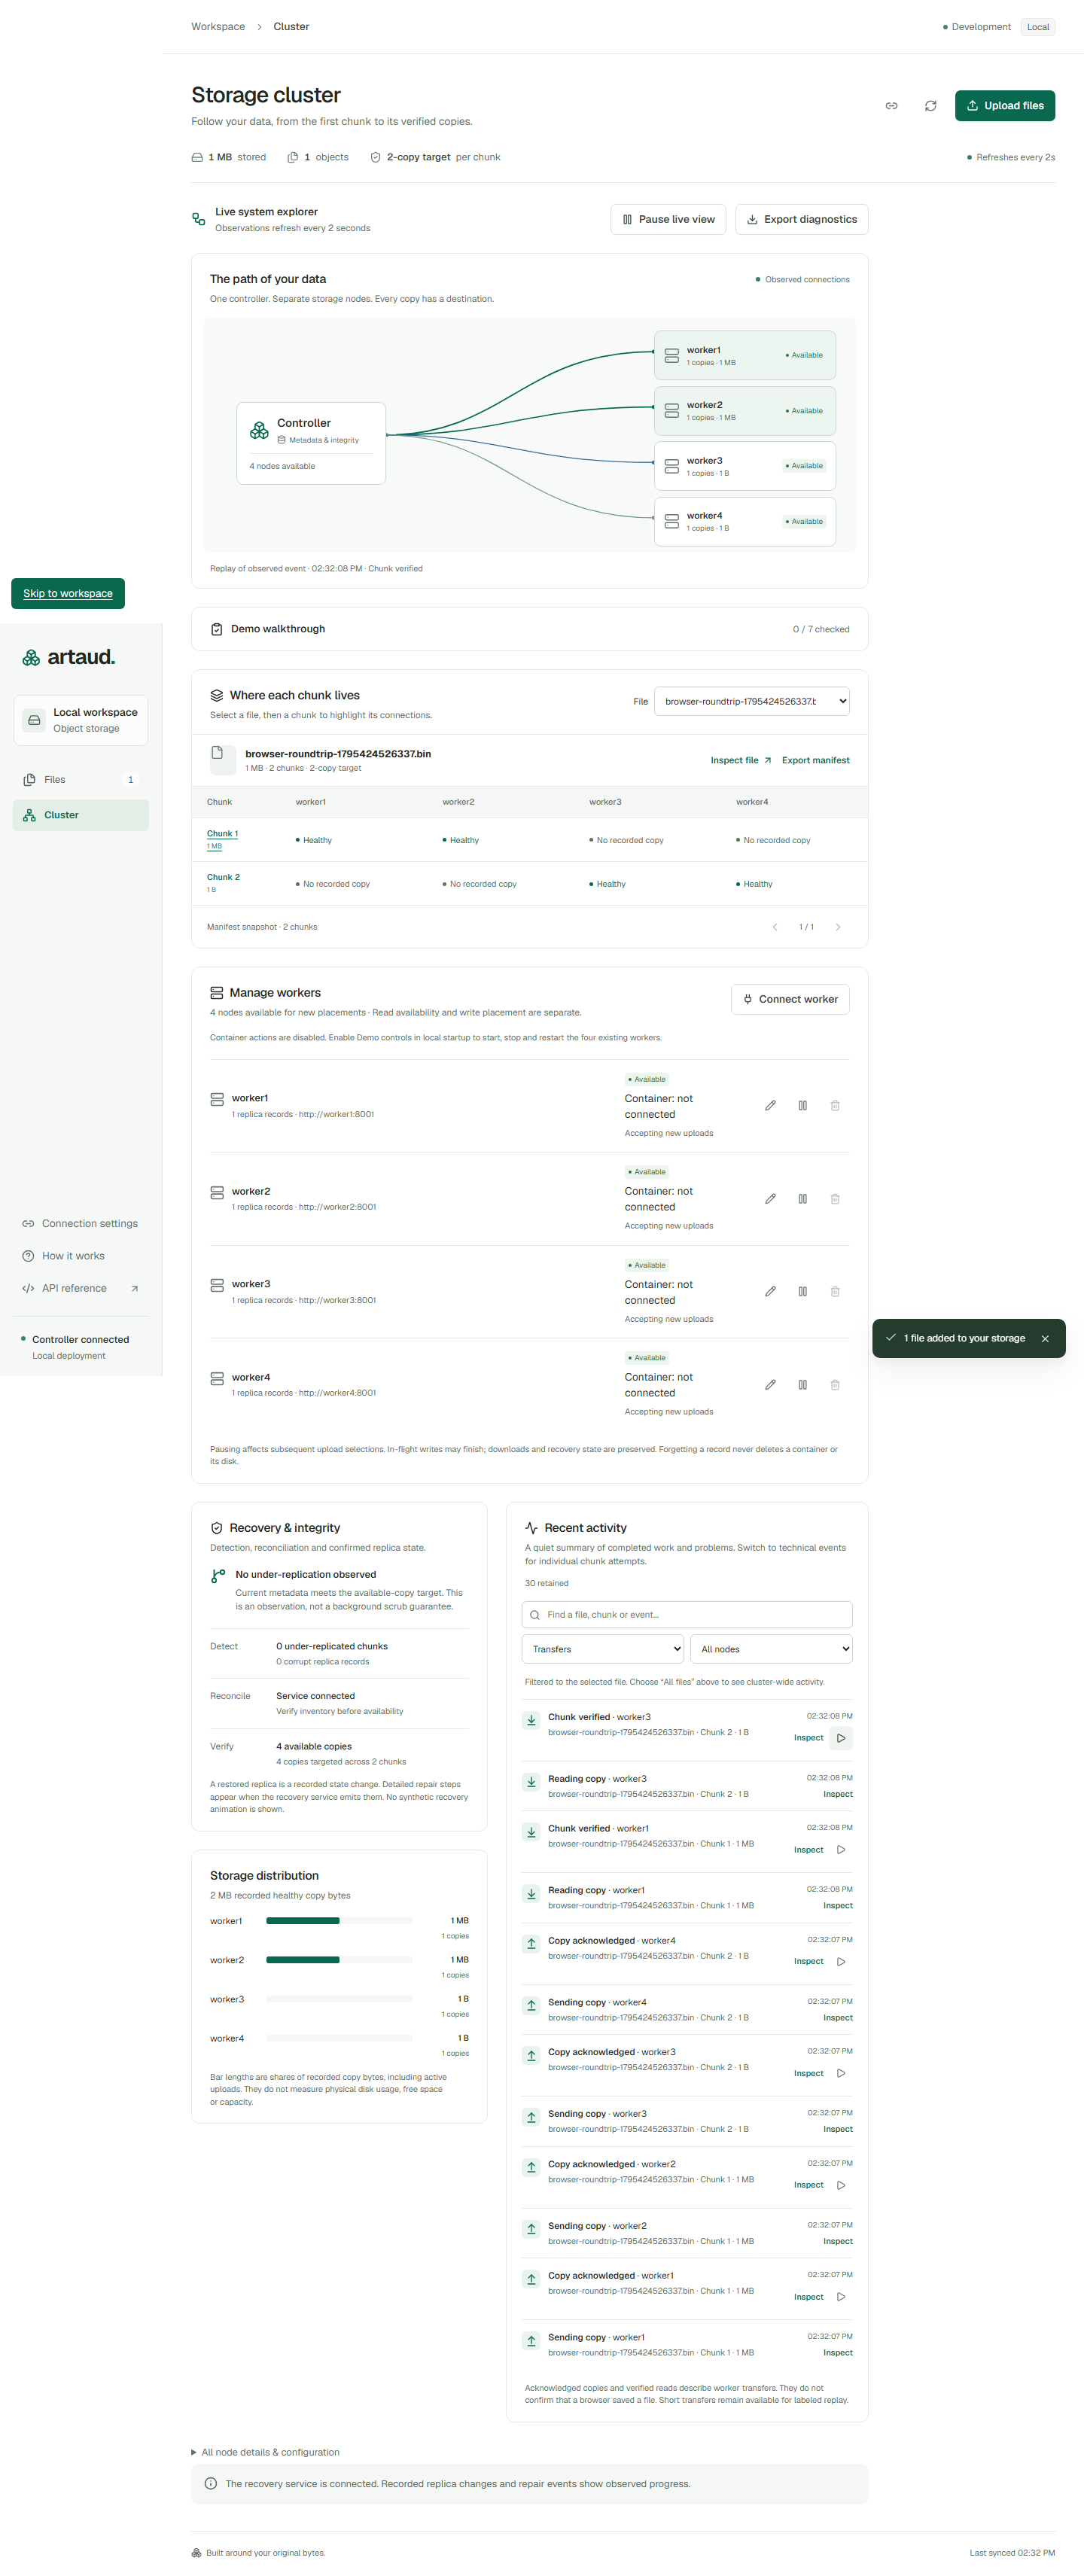
\includegraphics[
  width=.90\linewidth, viewport=228 2170 1195 3175, clip
]{figures/cluster.png}}
\end{center}
\endgroup

\figcaption{3}{The cluster view from the live acceptance run. The topology shows four admitted workers and the placement table shows separate holders for the two chunks of a synthetic upload. The screenshot is cropped to the topology and placement table.}

Open \textbf{Cluster} after an upload and select the object under
\textbf{Where each chunk lives}. Use the placement table to identify a worker
holding one copy before simulating an outage.

\clearpage
\reportsection{Inspecting an object}

\begingroup
\setlength{\fboxsep}{0pt}
\setlength{\fboxrule}{0.5pt}
\begin{center}
\fcolorbox{linegreen}{white}{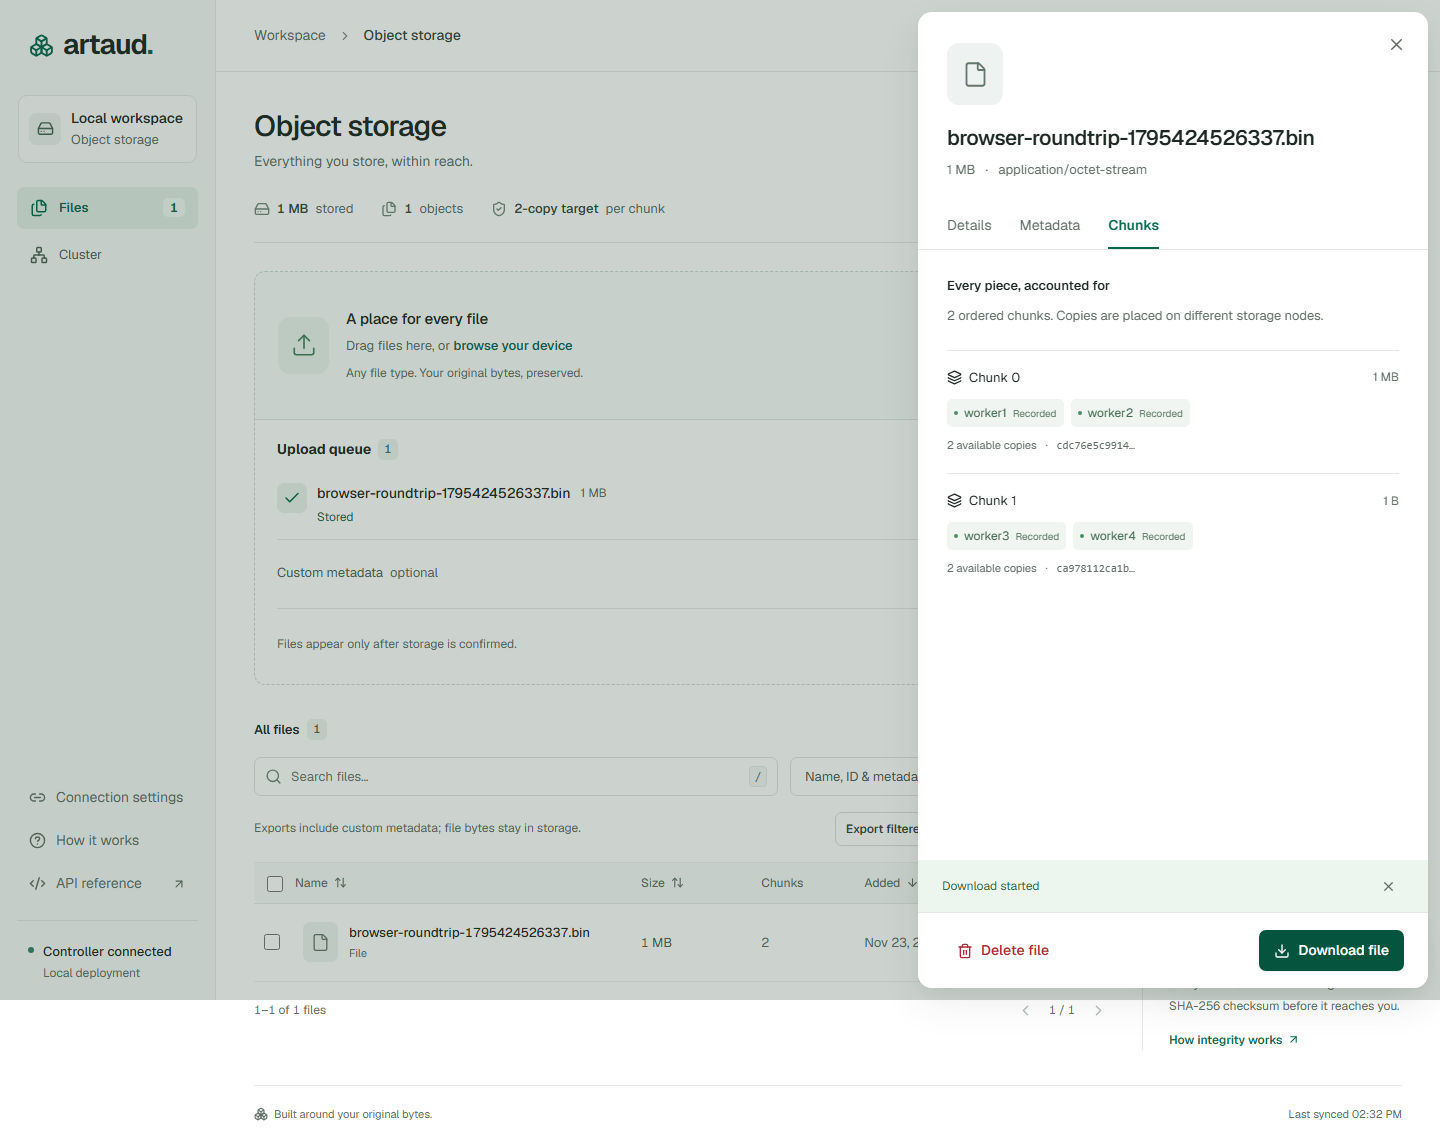
\includegraphics[
  width=.98\linewidth
]{figures/inspector.png}}
\end{center}
\endgroup

\figcaption{4}{The object inspector during the same live browser run.
The 1,000,001-byte upload produced a 1,000,000-byte chunk and a one-byte
tail. Each chunk shows two recorded locations.}

The \textbf{Details} tab shows the whole-object checksum and offers local
file verification. \textbf{Metadata} edits custom fields.
\textbf{Chunks} lists per-chunk hashes and worker locations. During a
demonstration, use the manifest to show which copies are affected by a
worker stop, then watch the placement and recovery views converge.

\topic{Demonstration sequence}
Upload a disposable file, inspect placement, then download and compare
the checksum. Stop \code{worker2}, download again with its surviving
counterpart, and wait for repair. Restart the worker and verify readmission.
With the demo overlay, inject corruption into a replica with a healthy
counterpart and observe verification and repair.

\clearpage
\reportsection{Verification and reproduction}

Validation used a clean snapshot of GitHub \code{master} at \code{\testedcommit}.
The five-container run used disposable containers and volumes. The existing
workspace data was outside that cluster.

\begin{tabularx}{\linewidth}{@{}p{40mm}X@{}}
\toprule
\textbf{Check} & \textbf{Result} \\
\midrule
Compose and builds & Base and demo overlay configurations validated. Controller and worker images and the frontend production build completed. \\
Backend suite & 369 passed. One opt-in live test was skipped here and run separately below. The suite emitted one Starlette test-client deprecation warning. \\
Frontend suite & 42 Vitest tests and 43 Chromium browser cases passed. \\
C1 and C2 & All four workers reached verified admission. A 5,000,001-byte object reconstructed to its original SHA-256 with two copies per chunk. \\
C4 & Reads survived a stop of \code{worker2}. Redundancy was restored, the worker rejoined and surplus copies were trimmed. A deliberately modified chunk and sidecar were detected and repaired. \\
C5 and API & Persistent restart, 50,000,000-byte upload and download, all six public operations and physical delete cleanup passed. \\
Live browser & A real browser uploaded through the controller, inspected the manifest, downloaded verified bytes and removed the synthetic object. \\
\bottomrule
\end{tabularx}

\topic{Run the same acceptance check}
From the repository root, build the two integration images as documented in
the README. Install the frontend dependencies and Chromium to include
browser verification. Run the check from the repository root.

{\small\begin{verbatim}
python tests/test_end_to_end.py --large --browser
\end{verbatim}}

For a manual demo, follow the README's \textit{Run locally} and
\textit{Demo checklist} sections. Use the controller API documentation at
\code{http://127.0.0.1:8000/docs} for route discovery.

\topic{Project references}
\begin{itemize}
\setlength{\itemsep}{2pt}
\item Assignment brief and project plan, under \code{docs/}.
\item Reproduction commands, architecture, and HTTP/SQLite contracts.
  \href{\repo/tree/20357e2c03212e9e3d8765286f69cbbbbfe62233}{Source snapshot}.
\end{itemize}

\end{document}
